\chapter{Planificación}
\label{chapter:planificación}


\section{Fechas importantes}

\paragraph{}
A continuación se detallan las fechas clave del proyecto:

\begin{table}[h!]
	\centering{}
	\begin{tabular}{ l | c | c | r }
		\hline
		Nombre & Fecha de inicio & Fecha de fin & Duración \\
		\hline
		\hline
		Reunión inicial con el cliente & 22/09/20 & 22/09/20 & 1  \\
		\hline
		Redacción de objetivos & 23/09/20 & 27/09/20 & 5  \\
		\hline
		Análisis de mercado & 28/09/20 & 18/10/20 & 21  \\
		\hline
		Enriquecer el DataSet & 19/10/20 & 01/11/20 & 14 \\
		\hline
		Diseño del Modelo 1 & 02/11/20 & 15/11/20 & 14  \\
		\hline
		Diseño del Modelo 2 & 16/11/20 & 29/11/20 & 14  \\
		\hline
		Diseño del Modelo 3 & 30/11/20 & 13/12/20 & 14  \\
		\hline
		Redacción de conclusiones & 14/12/20 & 27/12/20 & 14  \\
		\hline
		Preparación de la Defensa & 28/12/20 & 01/01/21 & 5  \\
		\hline
	\end{tabular}
	\caption{\textit{Tabla de fechas clave del proyecto}.}
	\label{table:gant_tabla}
\end{table}

\section{Diagrama Gantt}

\paragraph{}
\begin{figure}[h!]
	\centering
	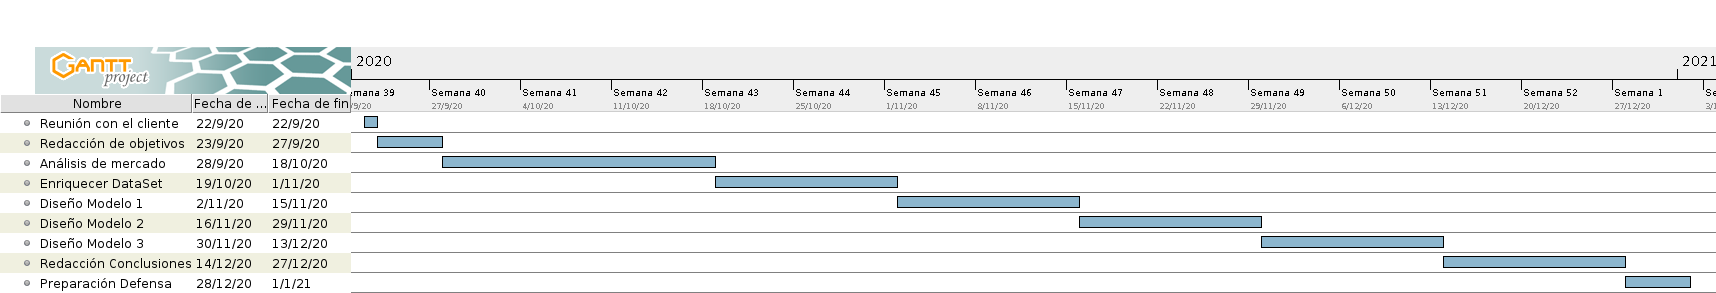
\includegraphics[width=0.9\textwidth]{figs/gant.png}
	\caption{Gantt del proyecto.}
	\label{fig:gant}
\end{figure}